% !TeX spellcheck = en_US
\addscenariosection[subsection]{1}{Castle Campaign $-$ The Queen's Gambit}{3. Two Knights Defense}{\images/catherine.png}

\begin{multicols*}{2}

\textbf{Author:} Tyson Heckert

\textbf{Source:} \href{https://travelledtales.com}{travelledtales.com}

\textit{With Vhidhax's stronghold in her grasp, Catherine needs to discover and halt the necromancer's next move.}

\subsection*{\MakeUppercase{Scenario length}}

This Scenario plays out over 8 Rounds.

\subsection*{\MakeUppercase{Player setup}}

\textbf{Faction:} Castle

\textbf{Faction Hero:} The same Hero you played in Scenario 2

\textbf{Starting Resources:} The resources you ended Scenario 2 with, plus 10 \svg{gold}

\textbf{Starting Income:} 10 \svg{gold}, 0 \svg{building_materials}, 0 \svg{valuables}

\textbf{Starting Units:} The army you ended Scenario 2 with

\textbf{Town Buildings:} \bronze\ Dwelling, \silver\ Dwelling, Citadel

\textbf{Bonus:} Begin the Scenario at Hero Level 3, but do not take new Ability Cards.

\subsection*{\MakeUppercase{AI Hero setup}}

\textbf{Faction:} Necropolis

\textbf{Enemy Army:} A Pack of Skeletons, a Pack of Zombies, a Pack of Liches, a Pack of Dread Knights

\textbf{Enemy Deck:} 3 × Might Cards, 3 × Magic Cards, 1 × Skill Card

\textbf{Enemy Spells:} 2 × Lightning Bolt, 1 × Curse

\textbf{Enemy Skills:} Cloak of the Undead King IV and VI, the enemy will play whichever it can

\subsection*{\MakeUppercase{Map setup}}

Take the following Map Tiles and arrange them as shown in the Scenario map layout:

\textbf{1 × Starting (I) Map Tile}
\begin{itemize}
    \item 1 × Necropolis (S1)
\end{itemize}

\textbf{2 × Far (II--III) Map Tile}
\begin{itemize}
    \item 2 × random Tiles from Necropolis or Dungeon (F1, F2, F4, F5, F7, F8)
\end{itemize}

\textbf{4 × Near (IV--V) Map Tile}
\begin{itemize}
    \item 2 × Necropolis (N1, N4)
    \item 2 × Dungeon (N2, N5)
\end{itemize}

\textbf{1 × Center (VI--VII) Map Tile}
\begin{itemize}
  \item 1 × Dragon Utopia Tile (C1)
\end{itemize}

\subsection*{\MakeUppercase{Heroes placement}}

Place your Castle Hero on the center Field of the Necropolis start Tile S1.

Place a Necropolis Hero on the bottom left Field of the leftmost Far Tile.
Reveal the Tile when the game begins.

\subsection*{\MakeUppercase{Victory Conditions}}

\begin{itemize}
  \item Defeat the enemy army
\end{itemize}


\subsection*{\MakeUppercase{Defeat Conditions}}
\begin{itemize}
  \item You lose one combat encounter
  \item You run out of time at the end of the 8th Round
\end{itemize}
\end{multicols*}

\begin{multicols}{2}

\subsection*{\MakeUppercase{Timed Events}}

\textbf{\nth{1} Round:}
\begin{itemize}
  \item Read ``The Race'' section
\end{itemize}

\textbf{When you complete the Scenario:}
\begin{itemize}
  \item Read ``Checkmate'' section
\end{itemize}

\subsection*{\MakeUppercase{Additional rules}}

During this Castle campaign Scenario, the following rules apply:

\begin{itemize}
  \item The Glory of Erathia building is unavailable.
  \item Each time you visit a Trading Post, draw the top Cards from the \bronze\ bronze, \silver\ silver, and \golden\ golden neutral enemy Decks.
  You may recruit any, or all of them by paying their cost.
  Shuffle any un-hired ones back into their Decks.

  \item After defeating the neutral army at the Dragon Utopia, add a random dragon from the \azure\ Azure neutral Deck to your army.
  \item The enemy army follows the normal AI movement rules, stopping to capture Settlements and Mines, with its ultimate goal to reach the Dragon Utopia.
  \item If the enemy army reaches the Dragon Utopia before you do, flip the Pack side of Dread Knights to Few and add a Pack of Ghost Dragons.
\end{itemize}

\begin{tikzpicture}[overlay]
    \node at (-1.0, -8.5) {
      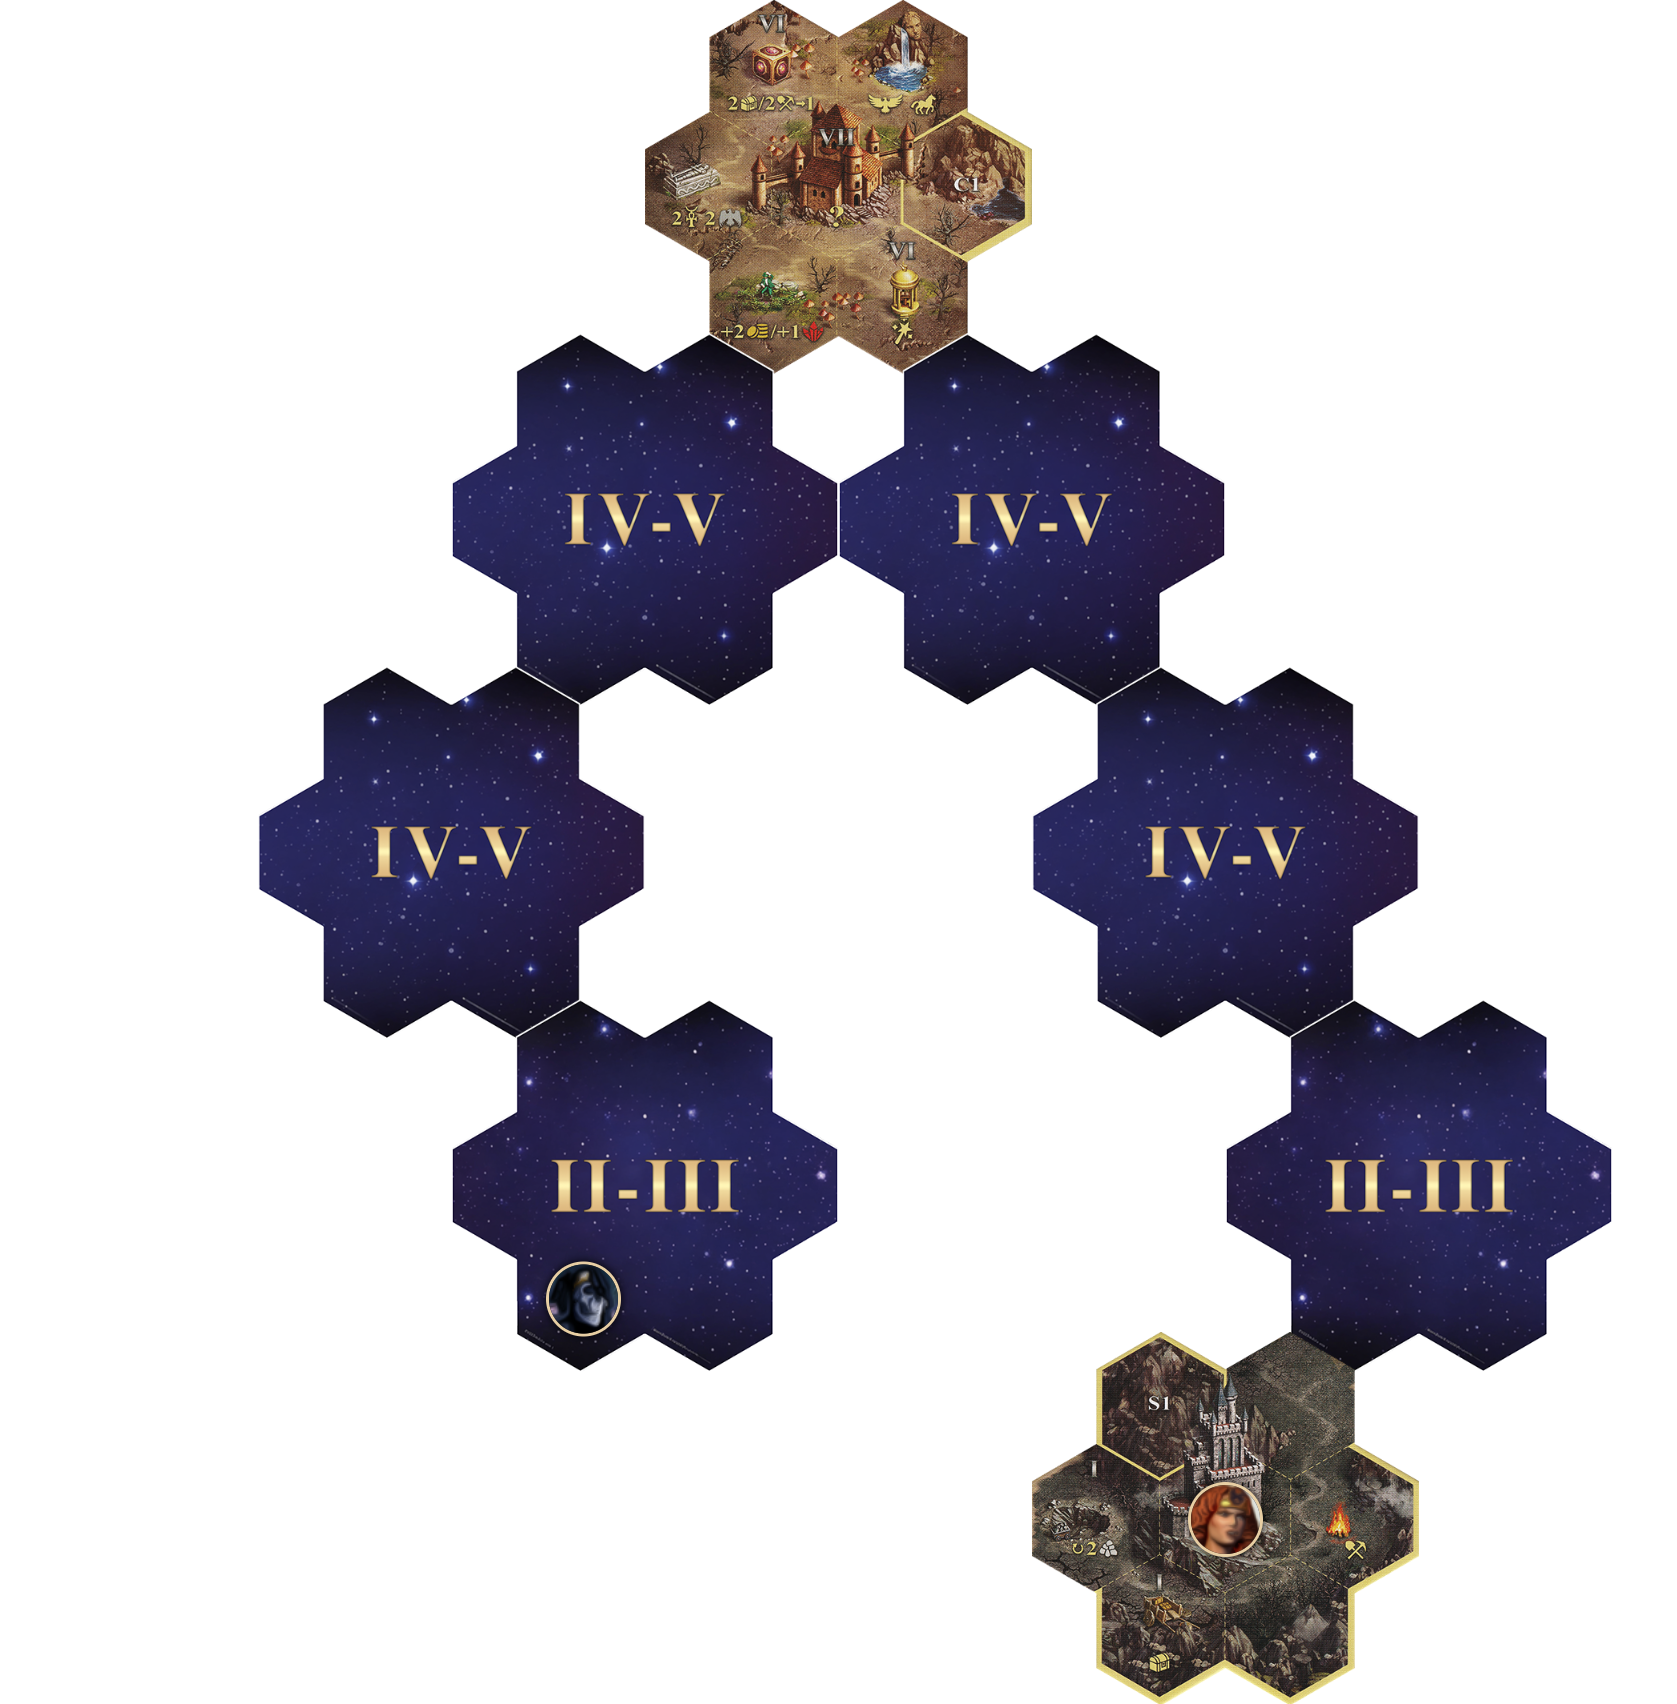
\includegraphics[width=0.70\paperwidth]{\_assets/maps/castle_two_knights_defense.png}
    };
  \end{tikzpicture}
\end{multicols}

\newpage

\begin{multicols*}{2}

\subsection*{\MakeUppercase{The story}}

\textbf{The Race}

Stacks of dry, cracked parchment sat next to dusty tomes on a table's blackened, rough-cut stone slab.
Catherine slumped over the numerous texts stashed throughout the necromancer's chambers while her eyes frantically scanned the pages.
She was searching for any clue to her enemy's plans.

After fruitless hours, she huffed and sent a moldering volume crashing through a stack of paper as exhaustion threatened to overcome her.
She was about to spin and leave the room when the corner of her eye caught a particular scribbling, revealed by her destructive act.
An ornate diagram, hastily scribbled, depicted what Catherine supposed might be some kind of necromantic summoning ritual.
Pulling the frail parchment closer, while most of it didn't make sense to her, it didn't take a mage to know what the dark drawings detailed.
They were the ritual instructions for raising Ghost Dragons from dead dragons.

Then it dawned on her.
Old tales told of an ancient Dragon Utopia in the badlands.
Vhidhax must be attempting to overtake the majestic creatures and use them against her in a last-ditch effort.
She frowned at the thought of her weakened enemy being able to defeat the dragons.
But if he did… If she missed something, he would have newfound strength enough to overpower her battered forces.
She clenched her fist, crushing the frail paper to dust before rushing to the doorway to gather who she could.

To her surprise, the necropolis' courtyard was abuzz with energy.
She placed her hands on the overlook's railing and peered over the edge to spy a host of knights in the color and flair of various baronies.

Rion came rushing up to her a moment later, intent on delivering news of their new guests.
``Queen Catherine!'' he said excitedly.
``Lordships around Steadwick heard of the tragedy and have sent their champions to aid us.
The knights spent days tracking and catching up to us, and they mean to join us and see the campaign through.''

Catherine smiled wide.
``Then tell them to get ready; the race is on.''

\textcolor{darkcandyapplered}{Add a Few Champions to your army.}

\textbf{Checkmate}

The broken remains of Vhidhax looked no grander than any of his many minions.
Necromantic energy had stripped the flesh from him long ago; without that power, his presence and ill-willed malevolence were gone as well.

Catherine wiped blood, sweat, and dirt from her face.
Rion had been right; the necromancer was not her father, but perhaps his slaying would ease the sting of her family discord and the sting of betrayal, at least a little.

Rion approached, and Catherine turned before embracing him in a rare moment of emotion.
The last time he'd seen his queen like this was when they were in Steadwick together, and he looked a little embarrassed as he was lost for words.
The two studied each other momentarily, silently checking on each other.
Rion thought she looked much older and weathered from the ordeal, but he was happy to see a twinkle in his queen's eyes again.

Her duty fulfilled and her seat secure, Catherine would see Steadwick rebuilt with Erathia just a little safer… for now.

\begin{itemize}
    \item \textcolor{darkcandyapplered}{If neither you or the enemy reached the Dragon Utopia, read ``A Queen's Right''}
    \item \textcolor{darkcandyapplered}{If the enemy army reached the Dragon Utopia before being defeated, read ``A Queen's Lament''}
    \item \textcolor{darkcandyapplered}{If you reached the Dragon Utopia and defeated the dragons within before defeating the enemy, read ``A Queen's Fury''}
\end{itemize}

\textbf{A Queen's Fury}

Catherine's hard eyes scanned the badlands from a window high on the Dragon Utopia.
While coming to blows with the famed dragon guardians was regrettable, she'd brought even them to heel, and the palace was hers.
No one would challenge her reign, not with the badlands under her control or the remaining dragons in her retinue.

Worn and tired faces looked up at her outside the fortress, like beggars asking for scraps.
What was left of who she'd brought into the hostile landscape was silently requesting the right to return home, yet the badlands were an enticing prize, and the bloodlust whipped up in the Queen of Erathia hadn't subsided yet.

It took much convincing from Rion before Catherine finally softened.
Reports from Steadwick were thrust in her face, and the mage's gentle nature reminded her that there were still those in her lands who needed her guidance.
So, finally, she ordered only a select few to watch over the badlands with the remaining mercenaries and dragons while she returned home with the rest.

\textbf{A Queen's Right}

A strange, deep calling swelled within Catherine.
She turned her focus to the majestic Dragon Utopia, with its rust-colored walls and pointed turrets.
It was an odd place for dragons to call home, yet its sheer presence was undeniable.

Catherine approached slowly, with the remains of her battered forces following cautiously.
Reaching the foot of the fortress, it was only a moment before the majestic snout of an azure dragon crawled into view from the large, curved, open entry to the stony fortress.
The rest of the creature soon followed, and with a stretch of wings, it stared down at the human queen.
While many fell to their knees, Catherine looked up to meet the dragon's gaze, and the two shared a moment of understanding between royalty.
It appeared the dragon knew what fate it had been spared from, and in thanks, it bowed to the human.
After a reflective moment, Catherine nodded, then turned, satisfied with the interaction.

His steed at a trot, Rion quickly approached.
``Well? Are we going inside?'' he asked curiously.

``There's no need,'' Catherine replied.
``I saw it in her eyes; the dragon knows what we did today.
We have their thanks and perhaps a favor to call on in the future.
Gods know we need it…''

Catherine drew her sword and reared her own steed high, presenting herself before her remaining forces with the dragon silhouetted behind her.
After a rousing speech that stirred the hearts of man and beast alike, she galloped to the rear lines to turn the formation toward home.

\textbf{A Queen's Lament}

Reality set in after the adrenaline and euphoria of a hard-fought victory wore off.
The battlefield was a nightmare of horrors.
Ghost Dragon corpses faded away as the last of their power died with them, and the scattered, broken bodies of both sides lay in clumps of gory remains.
The cost had been high…

Catherine regretted she couldn't save the dragons from their fate.
If things had been different, they might have been strong allies or at least sentinels to keep the local badland creatures in check.
Now, it was hard to tell what would leak from the unchecked wilds into other regions or townships under her charge.
Caution had won her the day, but she wondered if it was enough.
Would actions like this cause her downfall one day?

Home felt distant in the haze of fury that Catherine had been prisoner to.
As she trotted past the remains of those who had fought for her, her heart swelled with emotion.
It was war, and loss was inevitable.
She turned to the remaining few and threw a weak hand forward out of the badlands.
It was time to pick up the pieces.

\end{multicols*}
